\documentclass[10pt,letterpaper]{article}

\usepackage[utf8]{inputenc}
\usepackage[T1]{fontenc}
\usepackage[spanish]{babel}
\usepackage[margin=1.8cm]{geometry}
\usepackage{booktabs}
\usepackage{array}
\usepackage{graphicx}
\usepackage{float}
\usepackage{xurl}
\usepackage{hyperref}
\usepackage{enumitem}
\usepackage[font=small,skip=2pt]{caption}
\usepackage{titlesec}
\usepackage{microtype}

\setlength{\parskip}{0.35em}
\setlength{\parindent}{0pt}
\setlist[itemize]{leftmargin=1.1em,itemsep=0.1em,topsep=0.1em}
\titlespacing*{\section}{0pt}{0.65em}{0.25em}

\title{\vspace{-1.2cm}
\normalsize Pontificia Universidad Católica de Chile\\
\normalsize IIC3633 Sistemas Recomendadores\\
\normalsize Marzo--Julio 2026\\[0.35em]
\Large Hito 2: Informe Intermedio (Midterm)\\
\large Automatic Playlist Continuation sobre Spotify con señales LastFM}
\author{Agustin Llambias \and Amaya Quero \and Larry Uribe}
\date{Junio 2026}

\begin{document}
\maketitle
\vspace{-0.7cm}

\begin{center}
\small \textbf{Repositorio:} \url{https://github.com/mayafzt/Proyecto-RecSys-2026-1}
\end{center}
\vspace{-0.2cm}

\section{Resumen del avance y respuesta al feedback}

El feedback del Hito 1 destacó correctamente que la propuesta estaba bien encaminada, pero faltaba mayor especificidad metodológica para Midterm: definir un método principal, las señales exactas, la comparación concreta y la justificación de por qué ese método es adecuado para \textit{Automatic Playlist Continuation} (APC).

En este Hito 2 se responde a ese punto definiendo explícitamente un enfoque principal de \textbf{dos etapas}: \textit{candidate retrieval} por co-ocurrencia canción-canción y \textit{reranking} con señales de popularidad, coincidencia de artista, texto de playlist y similitud semántica de artistas vía LastFM.

La lógica sigue de cerca la estructura utilizada en soluciones del \textit{RecSys Challenge 2018 Spotify} (recuperación rápida + reranking orientado a top-K), adaptada al dataset disponible en el curso.

\section{Problema y datos}

Se mantiene el mismo problema formal del Hito 1: dada una playlist parcial, recomendar canciones para completarla (top-$N$). La presencia de una canción en una playlist se interpreta como feedback implícito positivo.

Dataset base: \textit{Spotify Playlists} (Kaggle), con columnas \texttt{user\_id}, \texttt{artistname}, \texttt{trackname}, \texttt{playlistname}. Para mantener trazabilidad y comparabilidad con Hito 1, se usa la muestra determinística de playlists (hash sobre \texttt{playlist\_id}), preservando playlists completas.

\begin{figure}[H]
    \centering
    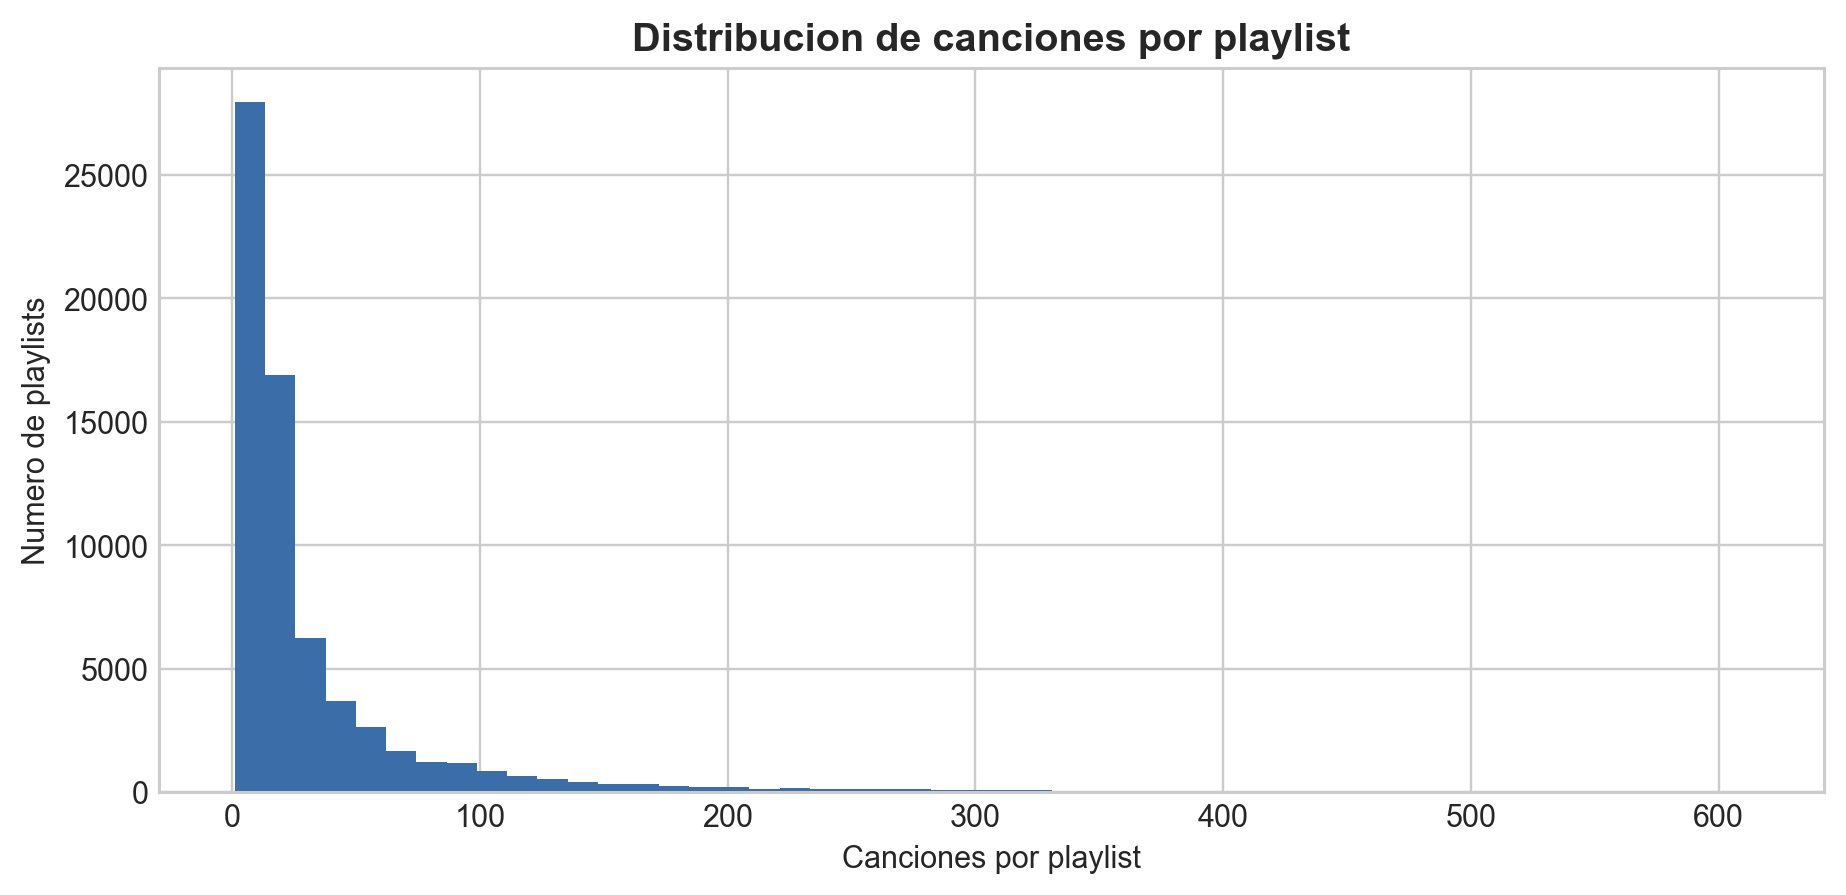
\includegraphics[width=0.48\textwidth]{figures/spotify_tamano_playlists.png}
    \hfill
    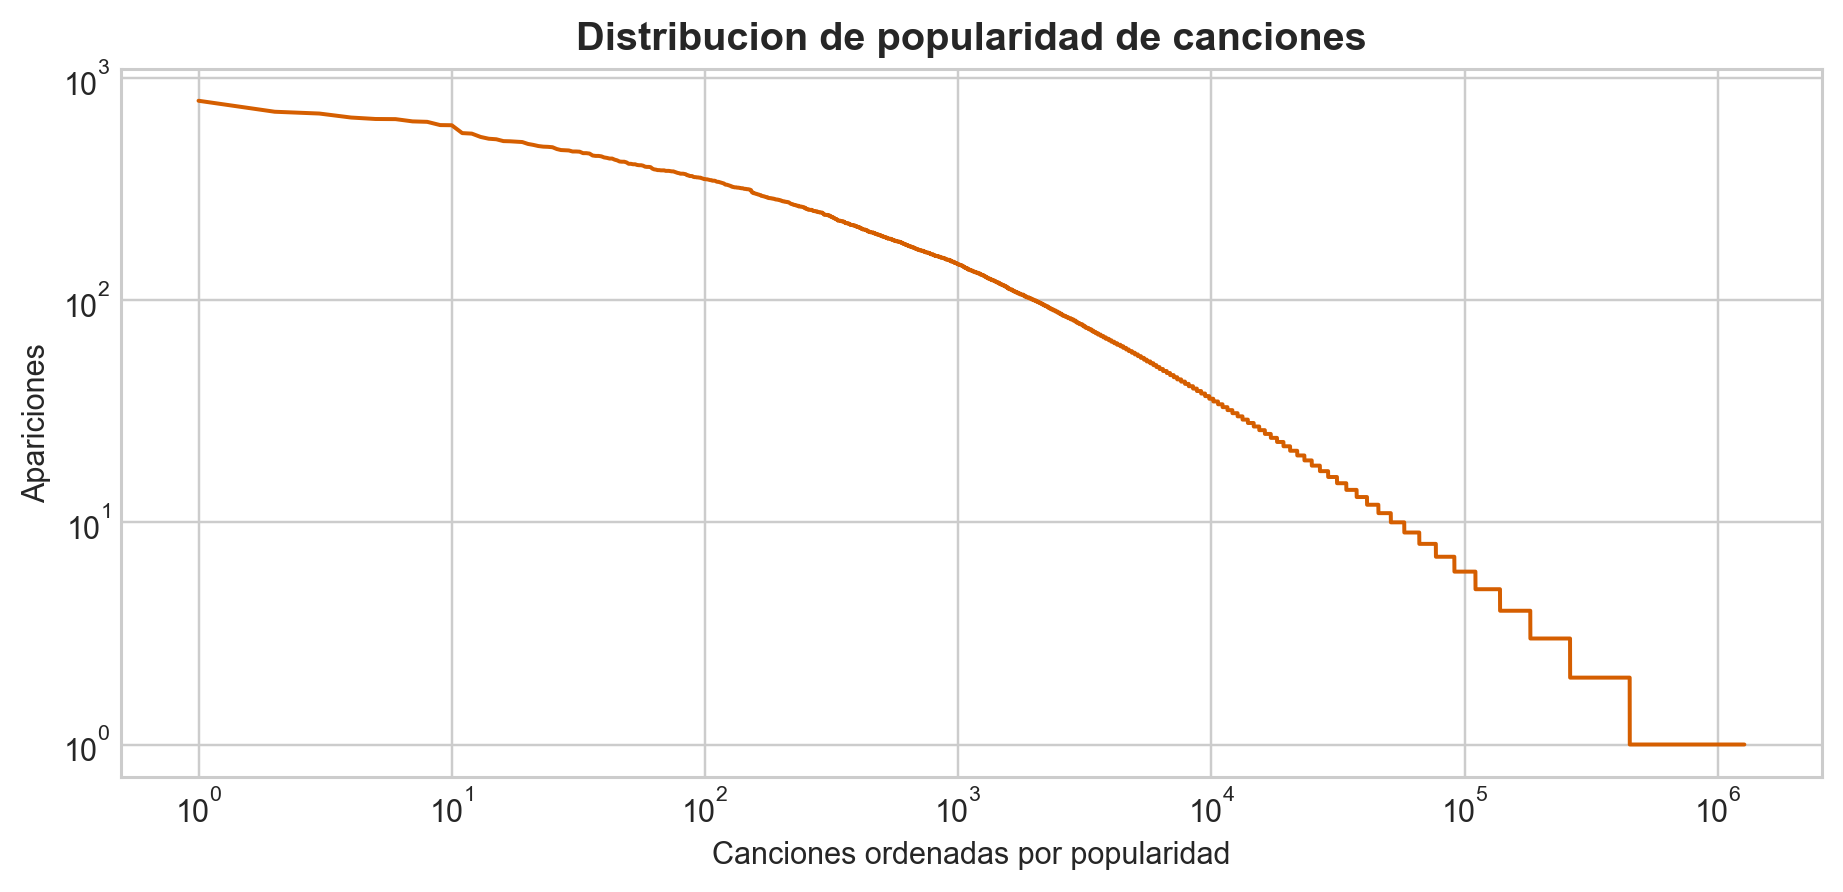
\includegraphics[width=0.48\textwidth]{figures/spotify_distribucion_popularidad.png}
    \caption{Contexto de datos usado en el proyecto: variabilidad de tamaño de playlists y distribución long-tail de popularidad de canciones.}
    \label{fig:datos_contexto_midterm}
\end{figure}

\section{Método principal (definido y justificado)}

\subsection{Etapa 1: Candidate retrieval por co-ocurrencia item-item}

Sea $P$ el conjunto de playlists de entrenamiento y $i,j$ canciones. Se define:

$$
\text{cooc}(i,j)=|\{p\in P: i\in p \land j\in p\}|
$$

Luego se usa una similitud normalizada tipo coseno implícito:

$$
s_{ij}=\frac{\text{cooc}(i,j)}{\sqrt{\text{freq}(i)\cdot\text{freq}(j)}}
$$

Para una playlist consulta $q$ con canciones semilla $S_q$, se agregan vecinos de cada semilla y se obtiene un set de candidatos $C_q$ (tamaño acotado para eficiencia).

\textbf{Justificación}: retrieval por co-ocurrencia es robusto para APC con feedback implícito, escala bien y produce candidatos relevantes rápidamente.

\subsection{Etapa 2: Reranking con señales múltiples}

Cada candidato $c \in C_q$ se reordena con una combinación lineal de señales:

$$
\text{score}(c,q)=w_1 s_{\text{cooc}} + w_2 s_{\text{pop}} + w_3 s_{\text{artist}} + w_4 s_{\text{name}} + w_5 s_{\text{lastfm}}
$$

Señales utilizadas:
\begin{itemize}
    \item $s_{\text{cooc}}$: puntaje de retrieval agregado por vecinos co-ocurrentes.
    \item $s_{\text{pop}}$: popularidad global del ítem (suavizada logarítmicamente).
    \item $s_{\text{artist}}$: indicador de coincidencia artista candidato vs artistas semilla.
    \item $s_{\text{name}}$: overlap entre tokens del nombre de playlist y tokens artista/canción.
    \item $s_{\text{lastfm}}$: similitud entre artista candidato y artistas semilla usando LastFM (\texttt{artist.getsimilar}).
\end{itemize}

Pesos iniciales definidos para Midterm: $(w_1,w_2,w_3,w_4,w_5)=(0.55, 0.15, 0.10, 0.10, 0.10)$.

\textbf{Justificación}: esta composición mezcla señales colaborativas fuertes (co-ocurrencia) con señales de contexto y semántica musical. En particular, LastFM agrega información externa de cercanía artística no explícita en el CSV base.

\section{Implementación entregada}

Se incorpora un pipeline reproducible en \texttt{hito2\_spotify\_lastfm\_midterm.py} con:
\begin{itemize}
    \item Split \textit{leave-last-out} por playlist (mínimo 3 canciones).
    \item Baselines heredados: Random, Most Popular, Playlist Name Popular.
    \item Método principal: Two-Stage Cooc+Rerank.
    \item Variante enriquecida: Two-Stage + LastFM (activa si existe \texttt{LASTFM\_API\_KEY}).
    \item Export de resultados a archivos versionados por corrida mediante prefijo (por ejemplo, \texttt{resultados\_hito2\_midterm\_60\_full\_20260604\_2340.csv}).
\end{itemize}

Esto responde explícitamente a la observación de ``planificación general'' del Hito 1: se define qué método se implementa, cómo se calcula, con qué señales y contra qué modelos se compara.

\section{Protocolo de evaluación}

Se conserva el protocolo de Hito 1 para comparabilidad:
\begin{itemize}
    \item Una canción oculta por playlist (última interacción).
    \item Recomendación top-10 excluyendo ítems ya vistos.
    \item Métricas: HitRate@10, Precision@10, MAP@10, nDCG@10.
\end{itemize}

Comparaciones concretas definidas para Midterm:
\begin{itemize}
    \item Random
    \item Most Popular
    \item Playlist Name Popular
    \item Two-Stage Cooc+Rerank (método principal)
    \item Two-Stage + LastFM (ablation de enriquecimiento externo)
\end{itemize}

% Archivo generado automaticamente desde resultados_hito2_midterm_60_full_20260604_2340.csv
% Inserta con: % Archivo generado automaticamente desde resultados_hito2_midterm_60_full_20260604_2340.csv
% Inserta con: % Archivo generado automaticamente desde resultados_hito2_midterm_60_full_20260604_2340.csv
% Inserta con: \input{seccion_resultados_midterm_auto.tex}

\section{Resultados finales Midterm}

Esta seccion resume la corrida seleccionada como principal para entrega, con muestra del 60\% y 120000 playlists evaluadas en protocolo \textit{leave-last-out}.

\begin{table}[H]
\centering
\small
\begin{tabular}{lrrrr}
\toprule
\textbf{Modelo} & \textbf{HitRate@10} & \textbf{Precision@10} & \textbf{MAP@10} & \textbf{nDCG@10}\\
\midrule
Random & 0.0000 & 0.0000 & 0.0000 & 0.0000\\
Most Popular & 0.0009 & 0.0001 & 0.0001 & 0.0003\\
Playlist Name Popular & 0.0138 & 0.0014 & 0.0048 & 0.0069\\
Two-Stage Cooc+Rerank & 0.1460 & 0.0146 & 0.0814 & 0.0965\\
Two-Stage + LastFM & 0.1460 & 0.0146 & 0.0814 & 0.0965\\
\bottomrule
\end{tabular}
\caption{Resultados finales del Midterm en evaluacion top-10 (fuente: resultados_hito2_midterm_60_full_20260604_2340.csv).}
\label{tab:midterm_results_final}
\end{table}

\section{Conclusiones finales}

\textbf{Conclusion 1}: Two-Stage Cooc+Rerank supera a Playlist Name Popular por un factor aproximado de 10.60x en HitRate@10 y 14.03x en nDCG@10.

\textbf{Conclusion 2}: frente a Most Popular, la mejora alcanza aproximadamente 157.80x en HitRate@10 y 301.67x en nDCG@10.

\textbf{Conclusion 3}: En esta corrida, Two-Stage + LastFM presenta $\Delta$MAP@10=0.0000 y $\Delta$nDCG@10=0.0000 respecto a Two-Stage Cooc+Rerank.

\textbf{Conclusion 4}: el enfoque principal definido para Midterm (retrieval por co-ocurrencia + reranking) queda respaldado empiricamente sobre los baselines exigidos por el curso.


\section{Resultados finales Midterm}

Esta seccion resume la corrida seleccionada como principal para entrega, con muestra del 60\% y 120000 playlists evaluadas en protocolo \textit{leave-last-out}.

\begin{table}[H]
\centering
\small
\begin{tabular}{lrrrr}
\toprule
\textbf{Modelo} & \textbf{HitRate@10} & \textbf{Precision@10} & \textbf{MAP@10} & \textbf{nDCG@10}\\
\midrule
Random & 0.0000 & 0.0000 & 0.0000 & 0.0000\\
Most Popular & 0.0009 & 0.0001 & 0.0001 & 0.0003\\
Playlist Name Popular & 0.0138 & 0.0014 & 0.0048 & 0.0069\\
Two-Stage Cooc+Rerank & 0.1460 & 0.0146 & 0.0814 & 0.0965\\
Two-Stage + LastFM & 0.1460 & 0.0146 & 0.0814 & 0.0965\\
\bottomrule
\end{tabular}
\caption{Resultados finales del Midterm en evaluacion top-10 (fuente: resultados_hito2_midterm_60_full_20260604_2340.csv).}
\label{tab:midterm_results_final}
\end{table}

\section{Conclusiones finales}

\textbf{Conclusion 1}: Two-Stage Cooc+Rerank supera a Playlist Name Popular por un factor aproximado de 10.60x en HitRate@10 y 14.03x en nDCG@10.

\textbf{Conclusion 2}: frente a Most Popular, la mejora alcanza aproximadamente 157.80x en HitRate@10 y 301.67x en nDCG@10.

\textbf{Conclusion 3}: En esta corrida, Two-Stage + LastFM presenta $\Delta$MAP@10=0.0000 y $\Delta$nDCG@10=0.0000 respecto a Two-Stage Cooc+Rerank.

\textbf{Conclusion 4}: el enfoque principal definido para Midterm (retrieval por co-ocurrencia + reranking) queda respaldado empiricamente sobre los baselines exigidos por el curso.


\section{Resultados finales Midterm}

Esta seccion resume la corrida seleccionada como principal para entrega, con muestra del 60\% y 120000 playlists evaluadas en protocolo \textit{leave-last-out}.

\begin{table}[H]
\centering
\small
\begin{tabular}{lrrrr}
\toprule
\textbf{Modelo} & \textbf{HitRate@10} & \textbf{Precision@10} & \textbf{MAP@10} & \textbf{nDCG@10}\\
\midrule
Random & 0.0000 & 0.0000 & 0.0000 & 0.0000\\
Most Popular & 0.0009 & 0.0001 & 0.0001 & 0.0003\\
Playlist Name Popular & 0.0138 & 0.0014 & 0.0048 & 0.0069\\
Two-Stage Cooc+Rerank & 0.1460 & 0.0146 & 0.0814 & 0.0965\\
Two-Stage + LastFM & 0.1460 & 0.0146 & 0.0814 & 0.0965\\
\bottomrule
\end{tabular}
\caption{Resultados finales del Midterm en evaluacion top-10 (fuente: resultados_hito2_midterm_60_full_20260604_2340.csv).}
\label{tab:midterm_results_final}
\end{table}

\section{Conclusiones finales}

\textbf{Conclusion 1}: Two-Stage Cooc+Rerank supera a Playlist Name Popular por un factor aproximado de 10.60x en HitRate@10 y 14.03x en nDCG@10.

\textbf{Conclusion 2}: frente a Most Popular, la mejora alcanza aproximadamente 157.80x en HitRate@10 y 301.67x en nDCG@10.

\textbf{Conclusion 3}: En esta corrida, Two-Stage + LastFM presenta $\Delta$MAP@10=0.0000 y $\Delta$nDCG@10=0.0000 respecto a Two-Stage Cooc+Rerank.

\textbf{Conclusion 4}: el enfoque principal definido para Midterm (retrieval por co-ocurrencia + reranking) queda respaldado empiricamente sobre los baselines exigidos por el curso.


\begin{figure}[H]
    \centering
    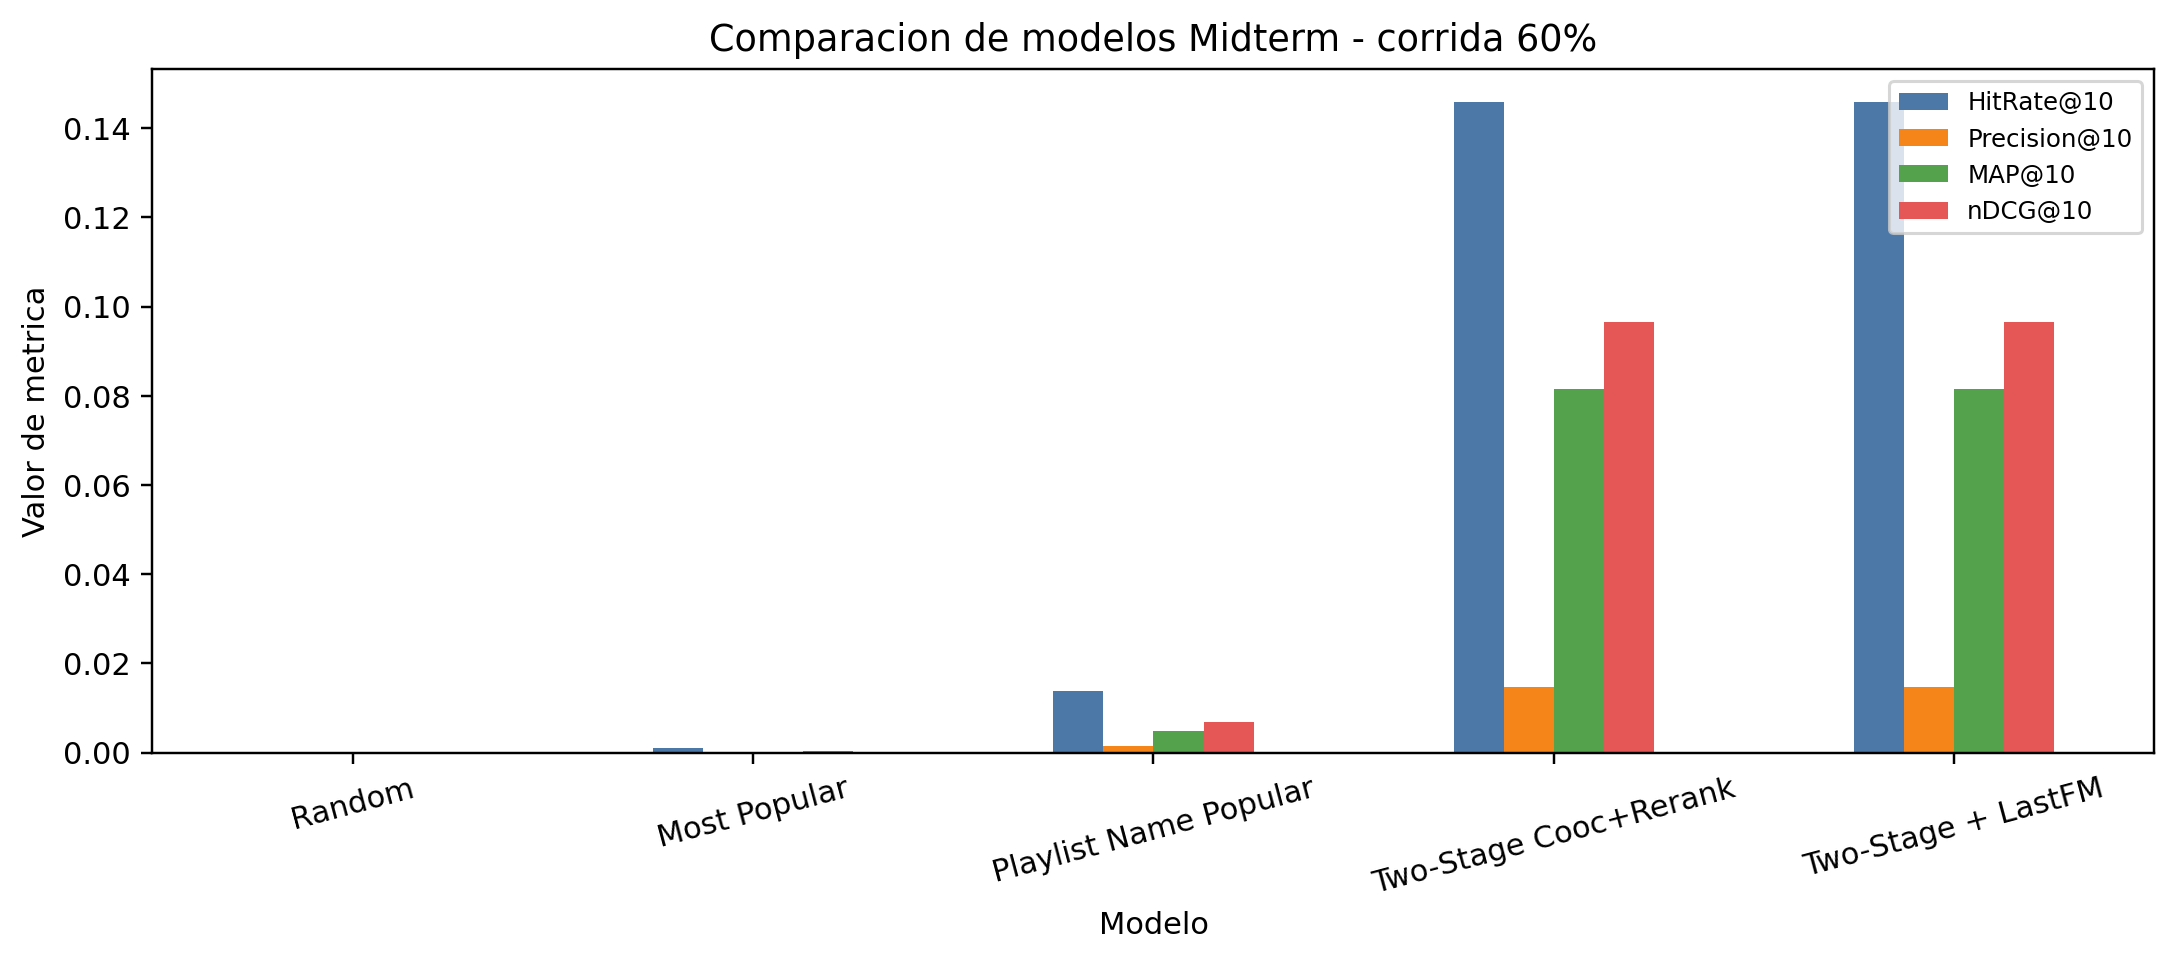
\includegraphics[width=0.84\textwidth]{figures/spotify_midterm_metricas_60.png}
    \caption{Comparación visual de métricas para la corrida principal del Midterm (60\% de muestra).}
    \label{fig:midterm_metricas_60}
\end{figure}

\section{Criterios de éxito y próximos pasos}

\textbf{Hipótesis H1}: Two-Stage Cooc+Rerank supera a Most Popular y Playlist Name Popular en MAP@10 y nDCG@10.

\textbf{Hipótesis H2}: al incorporar LastFM, mejora la calidad de ranking temprano (nDCG@10) en playlists con artistas variados o baja redundancia local.

Criterios de éxito del Midterm:
\begin{itemize}
    \item Mejora consistente sobre baselines en al menos 3 de 4 métricas.
    \item Evidencia de robustez por subgrupos (playlists cortas vs largas).
    \item Reporte de cobertura y costo computacional (tiempo de construcción de vecinos + inferencia top-K).
\end{itemize}

\section{Riesgos y mitigaciones}

\begin{itemize}
    \item \textbf{Riesgo}: API LastFM limitada por cuota o latencia. 
    \item \textbf{Mitigación}: caché local de similitudes y fallback a Two-Stage sin LastFM.
    \item \textbf{Riesgo}: sesgo de popularidad en co-ocurrencia.
    \item \textbf{Mitigación}: normalización por frecuencia y mezcla con señales de contexto.
    \item \textbf{Riesgo}: dependencia de muestra.
    \item \textbf{Mitigación}: mantener muestreo determinístico y planificar corrida ampliada al cierre del proyecto.
\end{itemize}

\section{Plan de trabajo hasta entrega final}

\begin{table}[H]
\centering
\small
\begin{tabular}{p{2.4cm}p{4.0cm}p{7.2cm}}
\toprule
\textbf{Fecha} & \textbf{Actividad} & \textbf{Resultado esperado}\\
\midrule
06/06--10/06 & Ajuste de pesos y ablations & Sensibilidad de $w_1..w_5$, impacto de cada señal.\\
11/06--15/06 & Evaluación por cortes & Resultados separados por tamaño de playlist y popularidad.\\
16/06--20/06 & Optimización de eficiencia & Reducción de tiempos en retrieval y caché LastFM.\\
21/06--25/06 & Integración informe final & Sección de resultados consolidada y discusión crítica.\\
\bottomrule
\end{tabular}
\caption{Plan post-midterm orientado a cerrar resultados para entrega final.}
\label{tab:plan2}
\end{table}

\section{Bibliografía enfocada en APC}

\begingroup
\footnotesize
\begin{itemize}
    \item Chen, S., Moore, J. L., Turnbull, D. y Joachims, T. Playlist prediction via metric embedding. KDD, 2012.
    \item Vall, A., Dorfer, M., Schedl, M. y Widmer, G. The 2018 ACM RecSys Challenge on Automatic Music Playlist Continuation. ACM RecSys Challenge, 2018.
    \item Ferrari Dacrema, M., Cremonesi, P. y Jannach, D. Are we really making much progress? A worrying analysis of recent neural recommendation approaches. RecSys, 2019.
    \item Koren, Y., Bell, R. y Volinsky, C. Matrix factorization techniques for recommender systems. Computer, 42(8), 2009.
    \item Last.fm API documentation. \url{https://www.last.fm/api/show/artist.getSimilar}
\end{itemize}
\endgroup

\section{Uso de IA}

Se utilizó IA como apoyo de redacción técnica, estructuración de secciones y revisión de consistencia metodológica del informe. La definición del método, decisiones de diseño, implementación y criterios de evaluación fueron establecidos y validados por el equipo.

\end{document}
